\section{Linux 下的 Shell 编程案例}

本次作业我设计并实现了一个基于 Bash Shell 的 Linux 命令答题系统。程序通过菜单提供开始答题、查看历史成绩、清空历史成绩和退出系统等功能，题目从外部题库文件中读取，答题结束后会把本次成绩保存到成绩文件中。这个案例既能练习 Linux 基础命令，也能体现 Shell 脚本中的条件判断、循环控制、函数封装、文件读写和程序调试等知识点。相比只演示单条命令，答题系统需要把输入、判断、统计、持久化和异常处理组织成完整流程，更能体现 Shell 脚本在 Linux 自动化任务中的作用。

\subsection{程序功能说明}

本程序的主要功能如下：

\begin{itemize}
    \item 显示主菜单，用户可以通过输入编号选择不同功能。
    \item 从 \cmd{questions.txt} 题库文件中逐行读取题目和标准答案。
    \item 判断用户输入是否为空、是否与标准答案一致，并根据结果计算得分和错误次数。
    \item 当答错次数达到设定上限时，系统自动结束本轮答题。
    \item 将每次答题的时间、得分、已答题数和错误题数保存到 \cmd{score.txt} 文件。
    \item 支持查看历史成绩，并使用 \cmd{awk} 统计历史最高分。
    \item 支持清空历史成绩，清空前需要用户再次确认，避免误操作。
\end{itemize}

程序采用“主菜单 + 功能函数”的结构，整体逻辑比较清晰。用户进入程序后，主循环会不断显示菜单，直到用户选择退出。每个功能被封装成独立函数，例如 \cmd{init\_env}、\cmd{show\_menu}、\cmd{start\_quiz}、\cmd{save\_score}、\cmd{show\_history} 和 \cmd{clear\_history}，这样可以减少重复代码。

\subsection{Shell 脚本执行方法}

在 Linux 平台下，可以进入脚本所在目录后执行以下命令运行程序：

\begin{minted}{bash}
cd task2
chmod +x linux_quiz.sh
./linux_quiz.sh
\end{minted}

其中，\cmd{chmod +x linux\_quiz.sh} 用于给脚本添加可执行权限，\cmd{./linux\_quiz.sh} 表示执行当前目录下的脚本文件。

\subsection{程序实现思路}

脚本整体采用函数化结构，把初始化环境、显示菜单、开始答题、保存成绩、查看历史成绩和清空历史成绩拆分为多个函数。主程序只负责循环显示菜单并根据用户选择调用对应函数，这样可以避免所有逻辑堆在一个长脚本中，也方便后续单独修改某个功能。

题库文件使用 \cmd{|} 作为题目和答案之间的分隔符，每一行表示一道题。答题函数通过 \cmd{while IFS='|' read -r question correct\_answer} 逐行读取题库，并使用独立文件描述符读取文件，避免用户输入和题库读取互相干扰。用户输入后，脚本会先去掉首尾空格，再判断是否为空、是否与标准答案一致，并更新分数、已答题数和错误次数。当错误次数达到上限时，当前轮答题自动结束。

成绩文件使用普通文本保存，每条记录包含答题时间、得分、已答题数和错误题数。查看历史成绩时，脚本使用 \cmd{awk} 从成绩文件中统计最高分；清空历史成绩前会要求用户输入确认，避免误删。这样既保持了脚本实现的简单性，也展示了 Shell 脚本对文本文件和命令行工具的组合能力。

\begin{figure}[H]
    \centering
    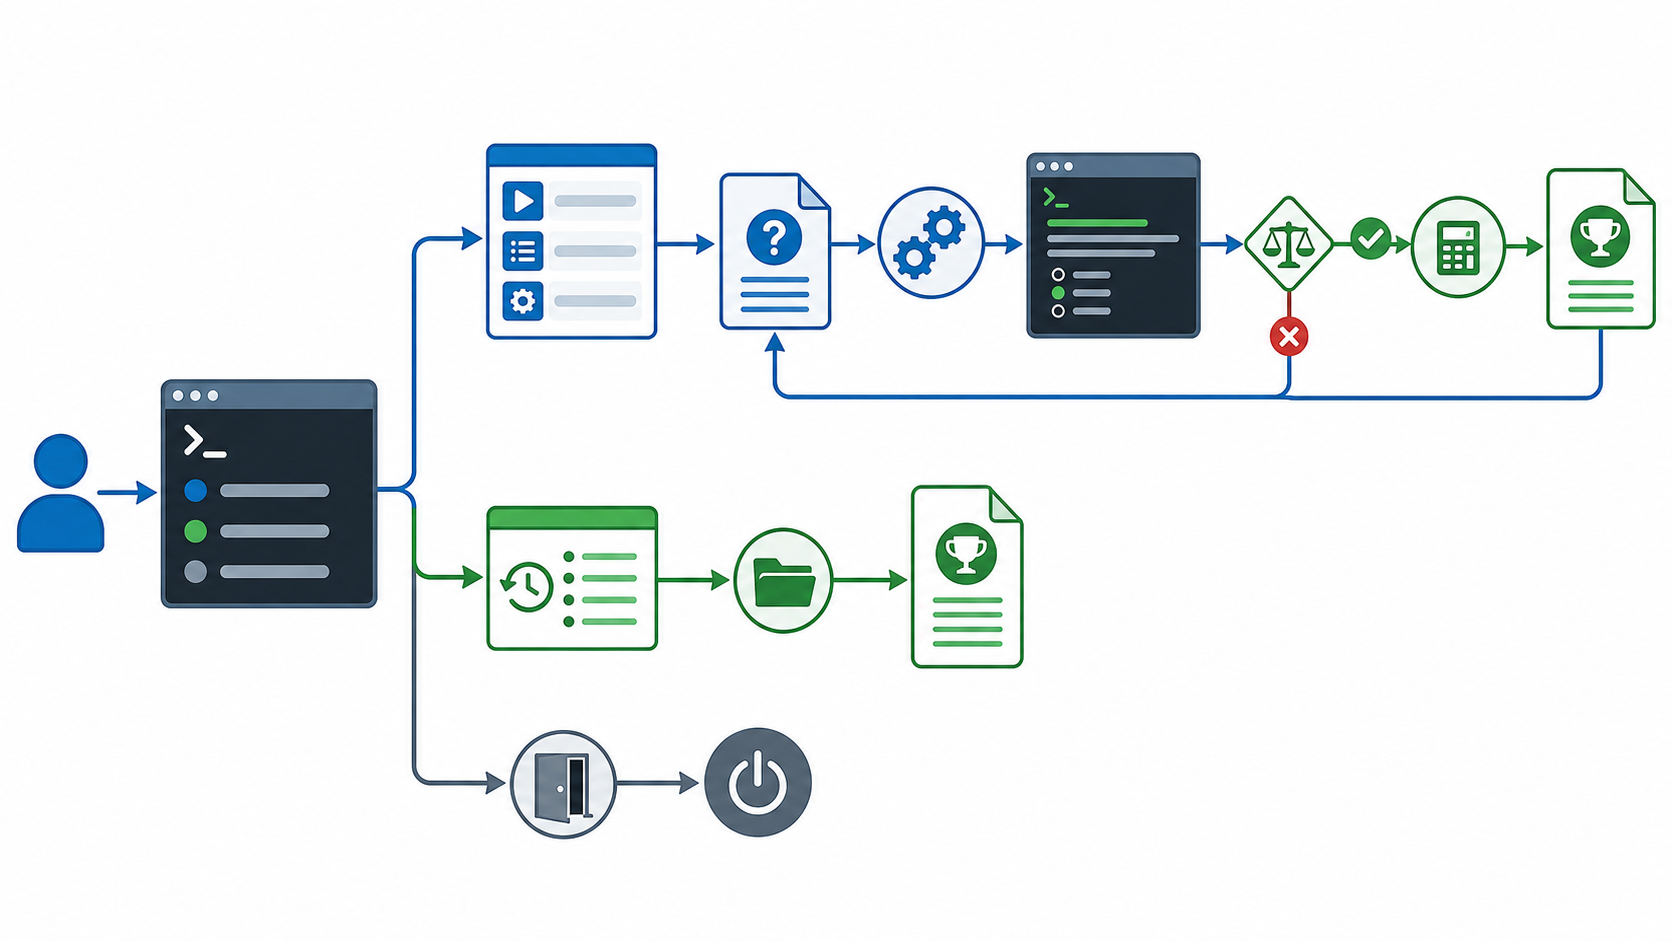
\includegraphics[width=0.85\textwidth]{pic/task2/Shell 答题系统流程图.png}
    \caption{Shell 答题系统流程示意图}
\end{figure}

从流程图可以看出，答题系统不是一次性执行完就退出的线性脚本，而是围绕主菜单形成循环。用户每次输入菜单编号后，脚本通过 \cmd{case} 分支调用对应函数；功能执行结束后再回到菜单，直到用户选择退出。这样的结构比较接近命令行小工具的常见写法，也便于后续继续扩展新功能。

\begin{table}[H]
    \centering
    \caption{Shell 脚本函数职责}
    \small
    \begin{tabular}{p{0.20\textwidth} p{0.34\textwidth} p{0.30\textwidth}}
        \toprule
        函数 & 主要职责 & 涉及的 Shell 知识点 \\
        \midrule
        \cmd{init\_env} & 检查题库文件和成绩文件，准备运行环境 & 文件判断、条件分支、重定向 \\
        \cmd{show\_menu} & 输出主菜单，提示用户选择功能 & \cmd{echo}、终端交互 \\
        \cmd{start\_quiz} & 读取题库、获取用户答案、判断正误、统计分数 & \cmd{while read}、字符串比较、计数变量 \\
        \cmd{save\_score} & 将本次成绩追加到成绩文件 & 输出重定向、日期命令、文本追加 \\
        \cmd{show\_history} & 显示历史成绩并统计最高分 & \cmd{cat}、\cmd{awk}、条件判断 \\
        \cmd{clear\_history} & 二次确认后清空成绩文件 & 用户输入、保护性判断、文件覆盖 \\
        \bottomrule
    \end{tabular}
\end{table}

\begin{table}[H]
    \centering
    \caption{程序文件格式说明}
    \small
    \begin{tabular}{p{0.18\textwidth} p{0.32\textwidth} p{0.34\textwidth}}
        \toprule
        文件 & 格式 & 作用 \\
        \midrule
        \cmd{linux\_quiz.sh} & Bash 脚本文件，包含函数和主循环 & 实现菜单、答题、判分、保存和异常处理 \\
        \cmd{questions.txt} & 每行一题，格式为“题目\cmd{|}答案” & 作为外部题库，便于不改脚本就扩展题目 \\
        \cmd{score.txt} & 每行一条成绩记录，包含时间、得分、题数和错误数 & 保存历史成绩，支持后续查看和统计最高分 \\
        \bottomrule
    \end{tabular}
\end{table}

把题库和成绩从脚本中拆出来，是这个案例中比较重要的设计选择。如果题目直接写在脚本里，每次新增题目都要修改程序逻辑；现在题库作为普通文本文件存在，只要保持分隔符格式一致，就可以继续追加题目。成绩文件同理，它不是复杂数据库，而是适合 Shell 处理的纯文本记录，因此可以直接用 \cmd{cat} 查看，也可以用 \cmd{awk} 做统计。

\subsection{案例展示}

与上一次基础命令作业一致，本次 Shell 脚本也在 Ubuntu 服务器上运行和测试，后续调试同样在这台服务器上完成。

首先创建一个目录来存放本次作业，然后放入 Shell 脚本文件和 \cmd{txt} 题库文件。

\begin{figure}[H]
    \centering
    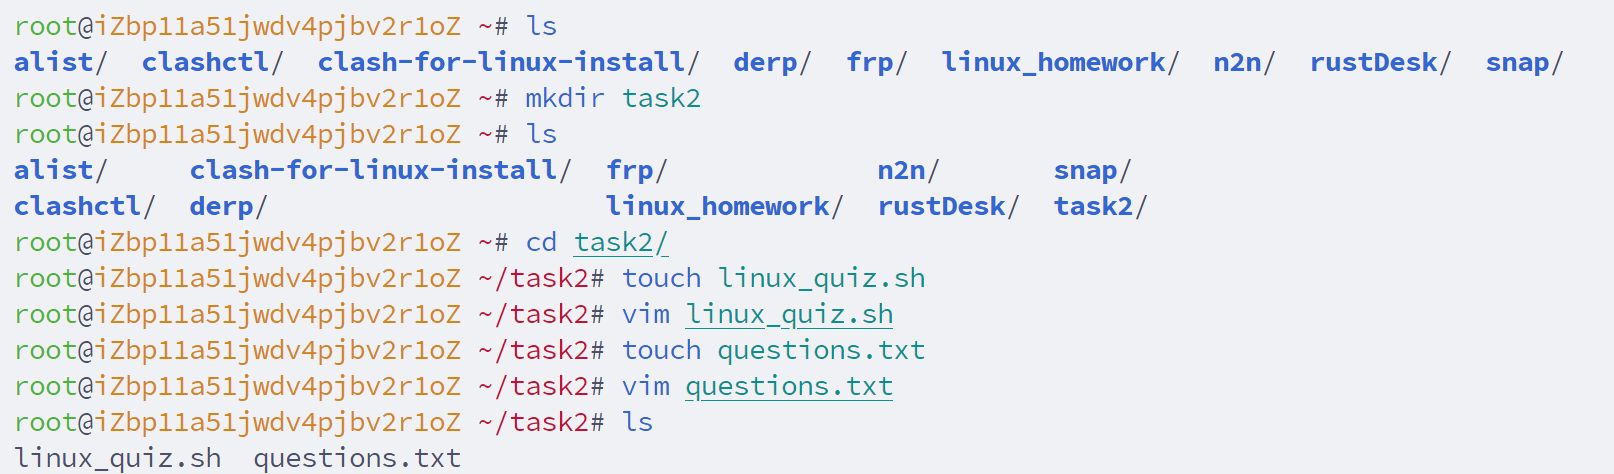
\includegraphics[width=0.8\textwidth]{pic/task2/image.png}
\end{figure}

随后按照前面的执行方法运行脚本。

主菜单页面：

\begin{figure}[H]
    \centering
    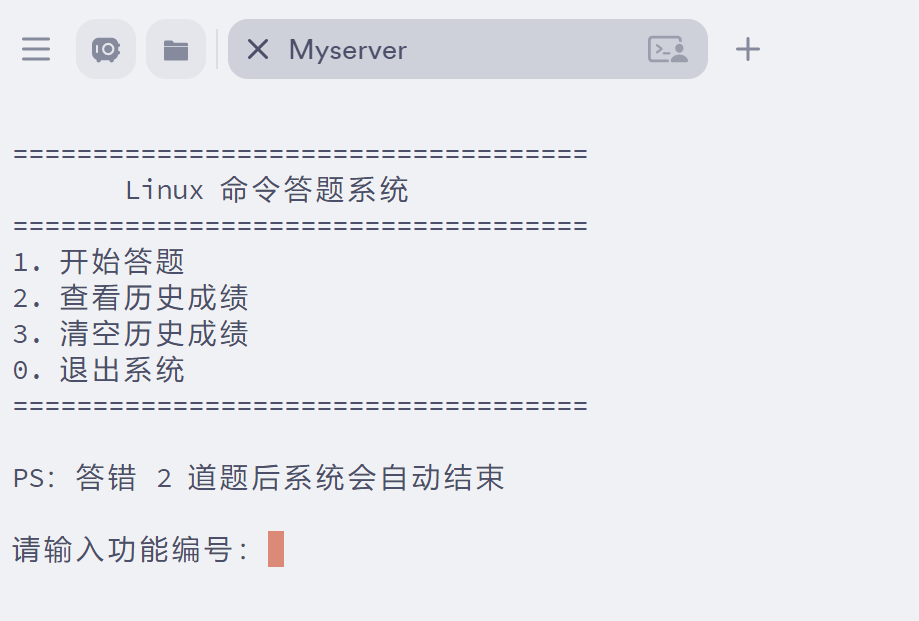
\includegraphics[width=0.8\textwidth]{pic/task2/image copy.png}
\end{figure}

开始答题界面：

\begin{figure}[H]
    \centering
    \begin{minipage}{0.48\textwidth}
        \centering
        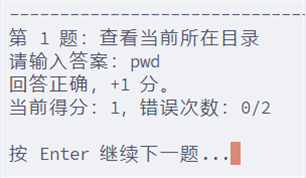
\includegraphics[width=\linewidth]{pic/task2/image copy 3.png}
    \end{minipage}
    \hfill
    \begin{minipage}{0.48\textwidth}
        \centering
        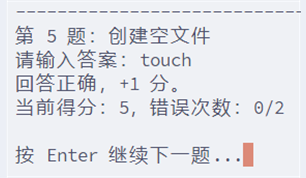
\includegraphics[width=\linewidth]{pic/task2/image copy 4.png}
    \end{minipage}

    \vspace{1em}

    \begin{minipage}{0.48\textwidth}
        \centering
        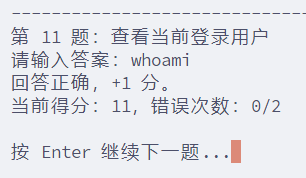
\includegraphics[width=\linewidth]{pic/task2/image copy 5.png}
    \end{minipage}
    \hfill
    \begin{minipage}{0.48\textwidth}
        \centering
        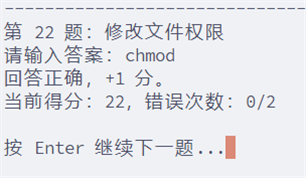
\includegraphics[width=\linewidth]{pic/task2/image copy 6.png}
    \end{minipage}
    \caption{答题界面}
\end{figure}



答题结束界面：

\begin{figure}[H]
    \centering
    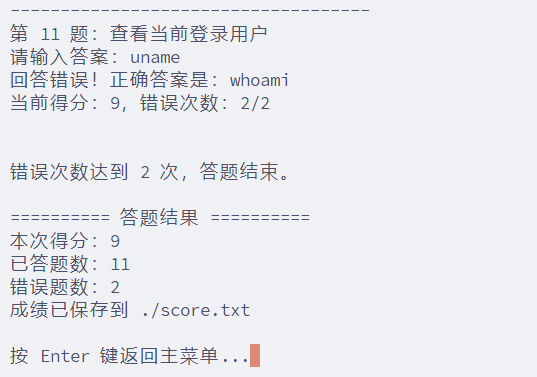
\includegraphics[width=0.8\textwidth]{pic/task2/image copy 2.png}
    \caption{答题结束界面}
\end{figure}

历史成绩界面：

\begin{figure}[H]
    \centering
    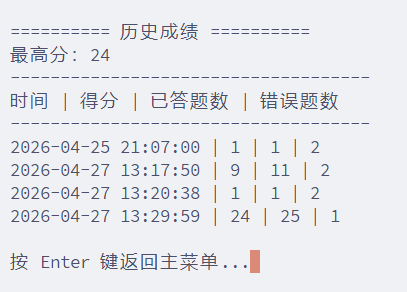
\includegraphics[width=0.8\textwidth]{pic/task2/image copy 7.png}
    \caption{历史成绩}
\end{figure}

题库和历史成绩都保存在当前目录下的 \cmd{txt} 文件中。目前题库包含 25 道题，后续如果需要扩展题库，可以直接在 \cmd{questions.txt} 文件中添加题目和答案，格式为“题目|答案”，每行一题。

\begin{figure}[H]
    \centering
    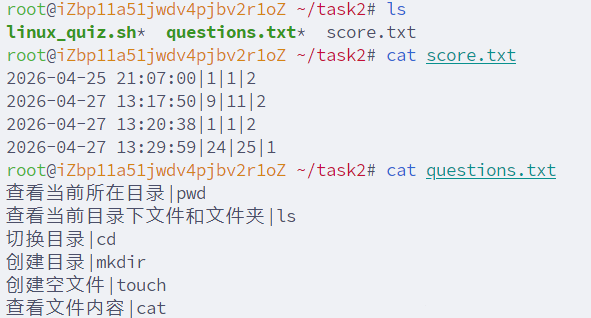
\includegraphics[width=0.8\textwidth]{pic/task2/image copy 8.png}
    \caption{题库和历史成绩文本文件}
\end{figure}

清空历史成绩时，程序会要求用户确认，可以选择确认清空或取消操作。

\begin{figure}[H]
    \centering
    \begin{minipage}{0.48\textwidth}
        \centering
        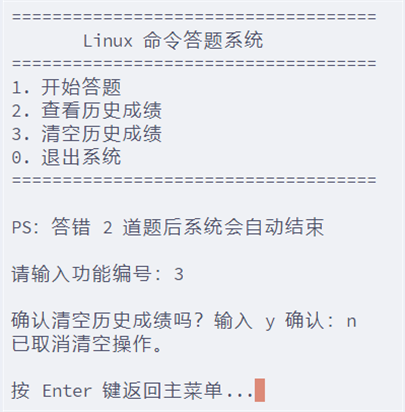
\includegraphics[width=\linewidth]{pic/task2/image copy 9.png}
    \end{minipage}
    \hfill
    \begin{minipage}{0.48\textwidth}
        \centering
        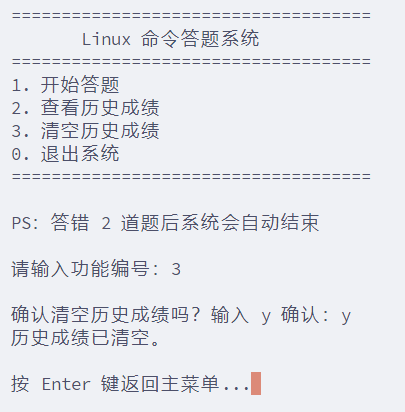
\includegraphics[width=\linewidth]{pic/task2/image copy 10.png}
    \end{minipage}
    \caption{清空历史成绩}
\end{figure}

退出系统。

\begin{figure}[H]
    \centering
    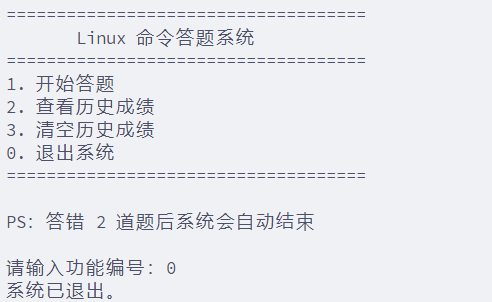
\includegraphics[width=0.8\textwidth]{pic/task2/image copy 11.png}
    \caption{退出系统}
\end{figure}


\subsection{Shell 程序调试方法}

在开发和调试 Shell 脚本时，我主要使用 \cmd{bash -n linux\_quiz.sh} 命令来检查脚本的语法错误。这个命令会解析脚本但不执行它，可以快速发现语法问题。

正常情况下，命令行没有输出，表示没有发现语法错误。

\begin{figure}[H]
    \centering
    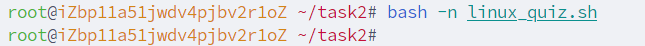
\includegraphics[width=0.8\textwidth]{pic/task2/image copy 12.png}
\end{figure}

如果有错误，会显示错误信息和所在行号，方便定位问题。

\begin{figure}[H]
    \centering
    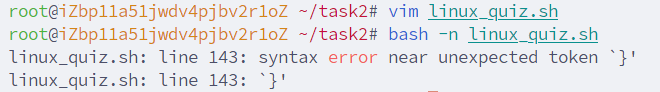
\includegraphics[width=0.8\textwidth]{pic/task2/image copy 13.png}
\end{figure}

使用 \cmd{vim} 打开脚本后可以看到，错误原因是分支结构中少了一个 \cmd{fi}，导致语法检查失败。补全该关键字后再次运行检查，脚本就不再报错。

\begin{figure}[H]
    \centering
    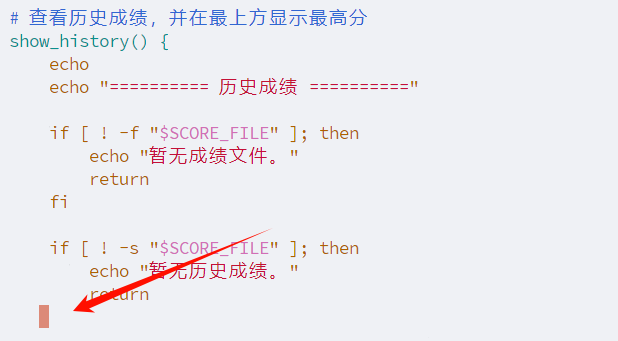
\includegraphics[width=0.8\textwidth]{pic/task2/image copy 14.png}
    \caption{错误修正}
\end{figure}

完成 Shell 脚本之后，可以使用 \cmd{bash -x linux\_quiz.sh} 来执行脚本并显示每条命令的执行过程，这样可以更细致地调试程序逻辑和变量值。

\begin{figure}[H]
    \centering
    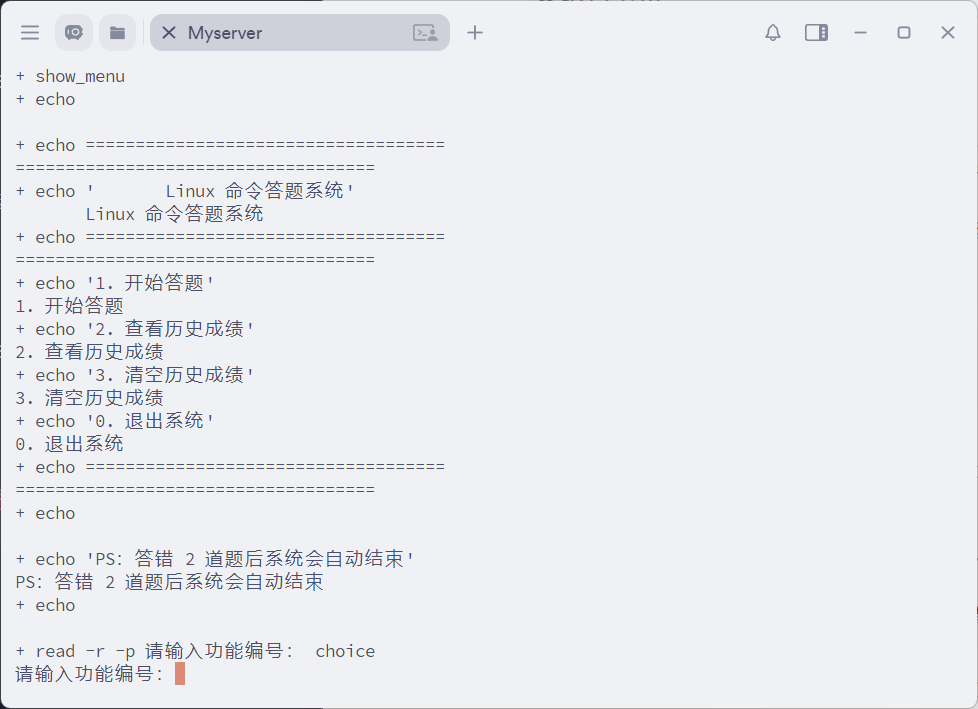
\includegraphics[width=0.8\textwidth]{pic/task2/image copy 15.png}
    \caption{执行跟踪调试}
\end{figure}

另外，我还构造了一些异常输入场景进行测试，例如删除 \cmd{questions.txt}、输入非法选项等，用来验证程序的健壮性和错误处理能力。

删除 \cmd{questions.txt} 后运行程序：

\begin{figure}[H]
    \centering
    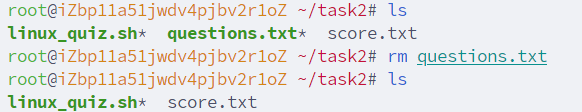
\includegraphics[width=0.8\textwidth]{pic/task2/image copy 16.png}
    \caption{删除题库文件}
\end{figure}

\begin{figure}[H]
    \centering
    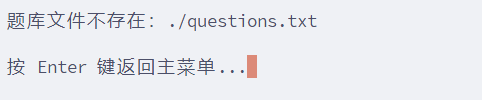
\includegraphics[width=0.8\textwidth]{pic/task2/image copy 17.png}
    \caption{运行程序}
\end{figure}

可以看出程序并没有崩溃，而是提示了题库文件不存在，说明程序的错误处理机制是有效的。

恢复题库文件后，答题输入中文选项：

\begin{figure}[H]
    \centering
    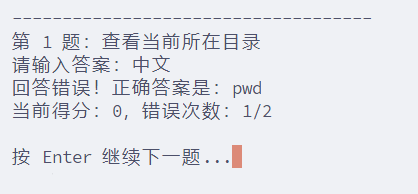
\includegraphics[width=0.8\textwidth]{pic/task2/image copy 18.png}
    \caption{输入中文选项}
\end{figure}

程序能够正确识别并说明该答案错误，说明程序对输入的处理也是正确的。

在主菜单页面输入非法选项时，程序不会崩溃，而是继续循环并提示用户输入正确选项。

\begin{figure}[H]
    \centering
    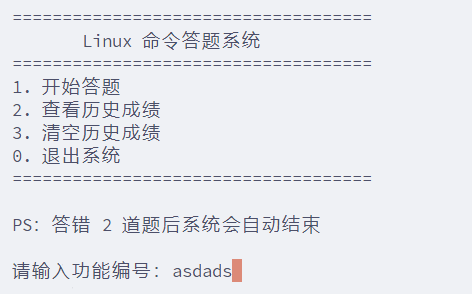
\includegraphics[width=0.8\textwidth]{pic/task2/image copy 19.png}
    \caption{输入非法选项}
\end{figure}

这些异常场景说明，脚本不仅要考虑“用户按预期输入”的情况，还要考虑文件缺失、输入为空、选项非法等常见问题。对于 Shell 程序而言，很多错误都不会自动变成清晰的异常对象，而是表现为命令返回非零状态、变量为空或文件读取失败。因此在关键位置增加文件存在性检查和输入判断，可以显著提高脚本的可用性。

\begin{table}[H]
    \centering
    \caption{异常输入与处理效果}
    \small
    \begin{tabular}{p{0.24\textwidth} p{0.30\textwidth} p{0.30\textwidth}}
        \toprule
        异常场景 & 程序处理方式 & 验证意义 \\
        \midrule
        题库文件缺失 & 输出提示并避免继续读取不存在的文件 & 验证文件检查逻辑有效 \\
        主菜单输入非法编号 & 提示用户重新输入，不退出程序 & 验证 \cmd{case} 默认分支有效 \\
        答题输入中文选项 & 按普通字符串处理并判断为错误答案 & 验证输入读取和字符串比较稳定 \\
        清空成绩前取消确认 & 不删除历史成绩 & 验证危险操作前的二次确认 \\
        成绩文件为空 & 仍能进入历史成绩功能并给出合理提示 & 验证查看历史时的边界情况 \\
        \bottomrule
    \end{tabular}
\end{table}

\subsection{脚本可维护性分析}

从可维护性角度看，这个答题系统虽然规模不大，但已经具备了几个比较好的脚本结构。首先，功能被拆分成多个函数，主循环只负责菜单分发，使脚本入口保持清晰。其次，题库和成绩使用外部文本文件保存，数据和程序逻辑没有混在一起。再次，清空历史成绩这种危险操作加入确认步骤，降低了误操作风险。

如果后续继续扩展，可以优先保持现有的函数化结构。例如增加随机抽题时，可以新增一个题目选择函数；增加错题本时，可以新增一个错题保存文件；增加排行榜时，可以在现有成绩文件基础上使用 \cmd{sort}、\cmd{awk} 等命令统计。这样扩展不会破坏已有菜单，也不需要重写全部答题流程。

\subsection{菜单循环与数据流分析}

这个 Shell 程序的主干是菜单循环。菜单循环的好处是用户可以反复执行不同功能，而不需要每次都重新启动脚本。用户选择开始答题后，程序进入答题流程；选择查看历史成绩后，程序读取成绩文件；选择清空历史成绩后，程序先确认再清空；选择退出后，循环结束。

\begin{table}[H]
    \centering
    \caption{菜单选项与数据流}
    \small
    \begin{tabular}{p{0.18\textwidth} p{0.28\textwidth} p{0.36\textwidth}}
        \toprule
        菜单选项 & 读取的数据 & 写入或输出的结果 \\
        \midrule
        开始答题 & \cmd{questions.txt} 中的题目和答案 & 在终端显示题目，结束后把成绩写入 \cmd{score.txt} \\
        查看历史成绩 & \cmd{score.txt} 中的历史记录 & 在终端输出历史记录，并统计最高分 \\
        清空历史成绩 & 用户确认输入 & 覆盖或清空 \cmd{score.txt}，删除历史记录内容 \\
        退出系统 & 用户菜单选择 & 结束主循环，脚本正常退出 \\
        \bottomrule
    \end{tabular}
\end{table}

从数据流角度看，题库文件是输入数据，成绩文件是输出数据，终端既是输入界面也是输出界面。用户通过 \cmd{read} 输入菜单编号和答案，脚本通过条件判断和循环控制决定下一步操作。这个结构虽然简单，但已经包含了交互式命令行程序的基本要素。

答题流程内部还有一层循环：外层菜单循环控制功能选择，内层题目循环逐行读取题库。内层循环每读到一行，就把分隔符左边作为题目，右边作为标准答案。用户输入答案后，脚本更新得分、已答题数量和错误次数。如果错误次数达到上限，内层循环提前结束，然后把本轮结果保存到成绩文件。


通过这个案例可以看到，Shell 脚本并不只适合写一两条自动化命令，也可以组织成有状态的交互程序。只要把数据文件、变量、循环和函数设计清楚，Shell 就能够完成比较完整的命令行应用。它的优势是直接利用 Linux 自带命令和文本文件，缺点是复杂数据结构和大型界面不如通用编程语言方便。

\subsection{实验小结}

这个 Shell 编程案例把前一节学到的基础命令进一步组织成了一个可交互的小程序。脚本中既有 \cmd{read} 获取用户输入，也有 \cmd{if} 和 \cmd{case} 完成分支判断，还有 \cmd{while} 循环读取题库文件，并通过重定向把成绩追加到文本文件中。相比单独练习命令，完整脚本更强调流程设计和异常处理。

通过调试过程可以看到，Shell 脚本虽然语法相对简洁，但对符号和结构非常敏感，例如缺少 \cmd{fi} 就会导致语法检查失败。因此在编写脚本时，先用 \cmd{bash -n} 检查语法，再用 \cmd{bash -x} 跟踪执行过程，是比较实用的调试方法。后续如果继续完善这个答题系统，还可以增加随机出题、错题记录、分数排行榜和题库合法性检查等功能。

\subsection{源代码与题库展示}

以下是本次 Shell 编程作业的主要源代码和配套题库文件。其中，\cmd{linux\_quiz.sh} 负责菜单交互、答题流程、成绩保存和异常处理，\cmd{questions.txt} 则保存题目与标准答案。题库文件采用“题目|答案”的格式组织，每行对应一道题。题库文件可以根据需要进行扩展，添加更多题目和答案。

\subsubsection{Shell 脚本}

\inputminted{bash}{code/task2/linux_quiz.sh}

\subsubsection{题库文件}

\inputminted{text}{code/task2/questions.txt}


